\documentclass[12pt]{article}
\usepackage{amsmath}
\usepackage{gensymb}
\usepackage{standalone}
\usepackage{graphicx}
\usepackage{tikz}
\usetikzlibrary{calc}
\usetikzlibrary{arrows}
\usetikzlibrary{decorations.pathreplacing}
\begin{document}

\section{Basic cone}

Below is a 2D representation of a light-cone. The mapping used is
to flatten the declination, showing the right-ascension ($\theta$):

\resizebox{\textwidth}{!}{\documentclass[crop,tikz]{standalone}
\usetikzlibrary{calc}
\usetikzlibrary{arrows}
\usetikzlibrary{decorations.pathreplacing}
\begin{document}
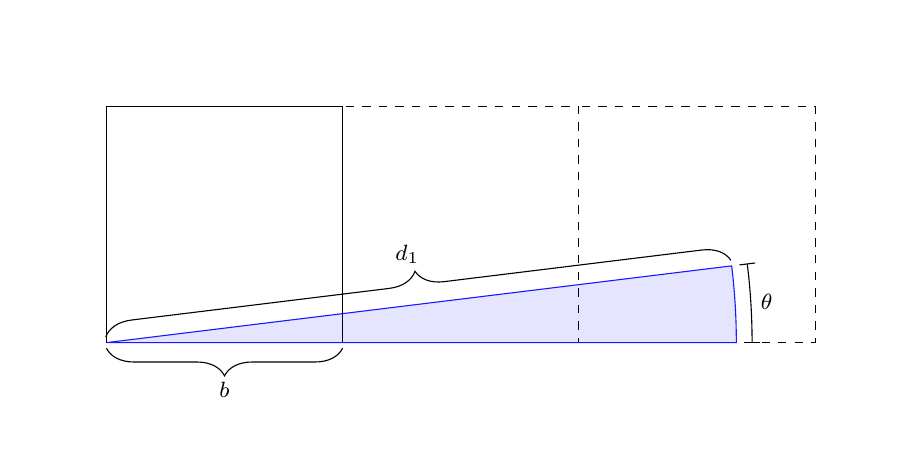
\begin{tikzpicture}
  % Constants
  \pgfmathsetmacro\b{3}
  \pgfmathsetmacro\d{8}
  \pgfmathsetmacro\t{7}
  \pgfmathsetmacro\a{0}
  % Boundary
  \path[use as bounding box] (0,0) rectangle (2+\b*3,2+\b);
  % Domain grids
  \draw (1,1) -- (1+\b,1) -- (1+\b,1+\b) -- (1,1+\b) -- cycle;
  \draw[dashed] (1+\b,1) -- (1+2*\b,1) -- (1+2*\b,1+\b) -- (1+\b,1+\b);
  \draw[dashed] (1+2*\b,1) -- (1+3*\b,1) -- (1+3*\b,1+\b) -- (1+2*\b,1+\b);
  % Domain size
  \draw[decorate,decoration={brace,mirror,amplitude=10pt},yshift=-2] (1,1) -- (1+\b,1) node [midway,yshift=-15] {\footnotesize $b$};
  % Lightcone
  \begin{scope}[shift={(1,1)}]
    \filldraw[fill=blue,fill opacity=0.1,draw=blue!90] (0,0) -- (\a:\d) arc (\a:\a+\t:\d) -- cycle;
    % Theta
    \draw (\a:\d+0.1) -- (\a:\d+0.3);
    \draw (\a+\t:\d+0.1) -- (\a+\t:\d+0.3);
    \draw (\a:\d+0.2) arc (\a:\a+\t:\d+0.2);
    \node at (\a+\t/2:\d+0.4) {\footnotesize $\theta$};
    % Length of d
    \draw[decorate,decoration={brace,amplitude=10pt},rotate=\a+\t,yshift=2] (0,0) -- (\d,0) node [midway,xshift=-4,yshift=16] {\footnotesize $d_1$};
  \end{scope}
\end{tikzpicture}
\end{document}
}

In generating unique cones, we want to place the cone entirely within
a single box in such a way that we can fit as many cones as possible,
while ensuring that no part of the cone overlaps any other part. Here is
what the cone looks like with no alterations:

\resizebox{\textwidth}{!}{\documentclass[crop,tikz]{standalone}
\usetikzlibrary{calc}
\usetikzlibrary{arrows}
\usetikzlibrary{decorations.pathreplacing}
\begin{document}
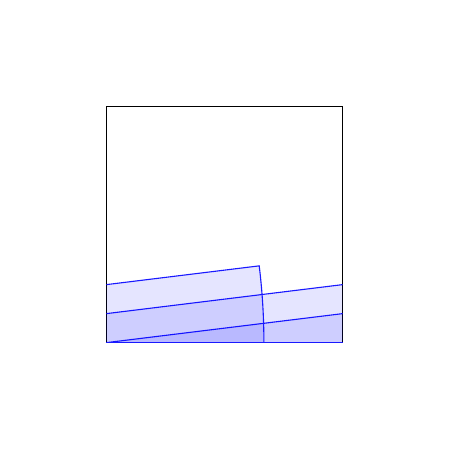
\begin{tikzpicture}
  % Constants
  \pgfmathsetmacro\b{3}
  \pgfmathsetmacro\d{8}
  \pgfmathsetmacro\t{7}
  \pgfmathsetmacro\a{0}
  % Boundary
  \path[use as bounding box] (0,0) rectangle (2+\b,2+\b);
  % Domain grids
  \draw (1,1) -- (1+\b,1) -- (1+\b,1+\b) -- (1,1+\b) -- cycle;
  % Lightcone
  \begin{scope}[shift={(1,1)}]
    \clip (0,0) rectangle(\b,\b);
    \filldraw[fill=blue,fill opacity=0.1,draw=blue!90] (0,0) -- (\a:\d) arc (\a:\a+\t:\d) -- cycle;
  \end{scope}
  \begin{scope}[shift={(1-\b,1)}]
    \clip (\b,0) rectangle(2*\b,\b);
    \filldraw[fill=blue,fill opacity=0.1,draw=blue!90] (0,0) -- (\a:\d) arc (\a:\a+\t:\d) -- cycle;
  \end{scope}
  \begin{scope}[shift={(1-2*\b,1)}]
    \clip (2*\b,0) rectangle(3*\b,\b);
    \filldraw[fill=blue,fill opacity=0.1,draw=blue!90] (0,0) -- (\a:\d) arc (\a:\a+\t:\d) -- cycle;
  \end{scope}
\end{tikzpicture}
\end{document}
}

Clearly the cone is in overlap with itself. In order to avoid this
overlap, we rotate the cone using an additional angle:

\resizebox{\textwidth}{!}{\documentclass[crop,tikz]{standalone}
\usetikzlibrary{calc}
\usetikzlibrary{arrows}
\usetikzlibrary{decorations.pathreplacing}
\begin{document}
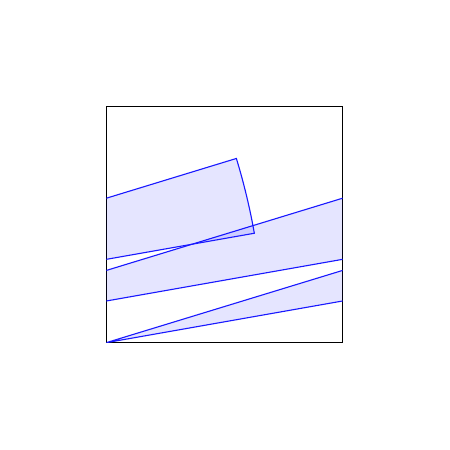
\begin{tikzpicture}
  % Constants
  \pgfmathsetmacro\b{3}
  \pgfmathsetmacro\d{8}
  \pgfmathsetmacro\t{7}
  \pgfmathsetmacro\a{10}
  % Boundary
  \path[use as bounding box] (0,0) rectangle (2+\b,2+\b);
  % Domain grids
  \draw (1,1) -- (1+\b,1) -- (1+\b,1+\b) -- (1,1+\b) -- cycle;
  % Lightcone
  \begin{scope}[shift={(1,1)}]
    \clip (0,0) rectangle(\b,\b);
    \filldraw[fill=blue,fill opacity=0.1,draw=blue!90] (0,0) -- (\a:\d) arc (\a:\a+\t:\d) -- cycle;
  \end{scope}
  \begin{scope}[shift={(1-\b,1)}]
    \clip (\b,0) rectangle(2*\b,\b);
    \filldraw[fill=blue,fill opacity=0.1,draw=blue!90] (0,0) -- (\a:\d) arc (\a:\a+\t:\d) -- cycle;
  \end{scope}
  \begin{scope}[shift={(1-2*\b,1)}]
    \clip (2*\b,0) rectangle(3*\b,\b);
    \filldraw[fill=blue,fill opacity=0.1,draw=blue!90] (0,0) -- (\a:\d) arc (\a:\a+\t:\d) -- cycle;
  \end{scope}
\end{tikzpicture}
\end{document}
}

While closer, there is still overlap. Again, with a larger angle:

\resizebox{\textwidth}{!}{\documentclass[crop,tikz]{standalone}
\usetikzlibrary{calc}
\usetikzlibrary{arrows}
\usetikzlibrary{decorations.pathreplacing}
\begin{document}
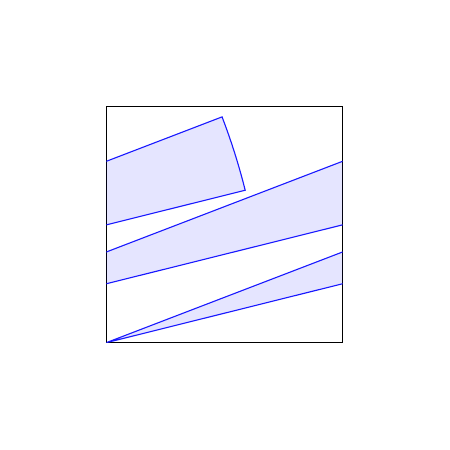
\begin{tikzpicture}
  % Constants
  \pgfmathsetmacro\b{3}
  \pgfmathsetmacro\d{8}
  \pgfmathsetmacro\t{7}
  \pgfmathsetmacro\a{14}
  % Boundary
  \path[use as bounding box] (0,0) rectangle (2+\b,2+\b);
  % Domain grids
  \draw (1,1) -- (1+\b,1) -- (1+\b,1+\b) -- (1,1+\b) -- cycle;
  % Lightcone
  \begin{scope}[shift={(1,1)}]
    \clip (0,0) rectangle(\b,\b);
    \filldraw[fill=blue,fill opacity=0.1,draw=blue!90] (0,0) -- (\a:\d) arc (\a:\a+\t:\d) -- cycle;
  \end{scope}
  \begin{scope}[shift={(1-\b,1)}]
    \clip (\b,0) rectangle(2*\b,\b);
    \filldraw[fill=blue,fill opacity=0.1,draw=blue!90] (0,0) -- (\a:\d) arc (\a:\a+\t:\d) -- cycle;
  \end{scope}
  \begin{scope}[shift={(1-2*\b,1)}]
    \clip (2*\b,0) rectangle(3*\b,\b);
    \filldraw[fill=blue,fill opacity=0.1,draw=blue!90] (0,0) -- (\a:\d) arc (\a:\a+\t:\d) -- cycle;
  \end{scope}
\end{tikzpicture}
\end{document}
}

This is an acceptable solution. However, it's not optimal. We could have
chosen a smaller angle, which would allow more cones to fit in the domain
(potentially). So, the question to be answered is, what angle should we
choose to give the optimal solution? If we examine the optimal solution
visually we might get some idea of a sufficient condition:

\resizebox{\textwidth}{!}{\documentclass[crop,tikz]{standalone}
\usetikzlibrary{calc}
\usetikzlibrary{arrows}
\usetikzlibrary{decorations.pathreplacing}
\begin{document}
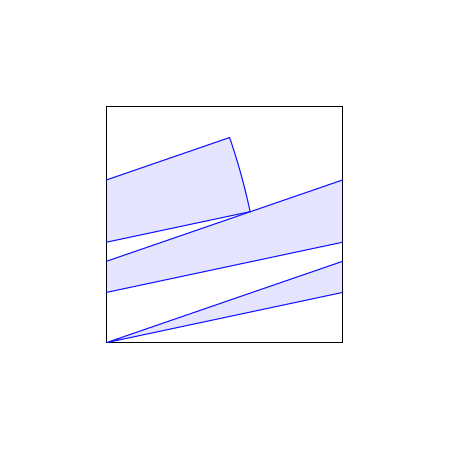
\begin{tikzpicture}
  % Constants
  \pgfmathsetmacro\b{3}
  \pgfmathsetmacro\d{8}
  \pgfmathsetmacro\t{7}
  \pgfmathsetmacro\a{12}
  % Boundary
  \path[use as bounding box] (0,0) rectangle (2+\b,2+\b);
  % Domain grids
  \draw (1,1) -- (1+\b,1) -- (1+\b,1+\b) -- (1,1+\b) -- cycle;
  % Lightcone
  \begin{scope}[shift={(1,1)}]
    \clip (0,0) rectangle(\b,\b);
    \filldraw[fill=blue,fill opacity=0.1,draw=blue!90] (0,0) -- (\a:\d) arc (\a:\a+\t:\d) -- cycle;
  \end{scope}
  \begin{scope}[shift={(1-\b,1)}]
    \clip (\b,0) rectangle(2*\b,\b);
    \filldraw[fill=blue,fill opacity=0.1,draw=blue!90] (0,0) -- (\a:\d) arc (\a:\a+\t:\d) -- cycle;
  \end{scope}
  \begin{scope}[shift={(1-2*\b,1)}]
    \clip (2*\b,0) rectangle(3*\b,\b);
    \filldraw[fill=blue,fill opacity=0.1,draw=blue!90] (0,0) -- (\a:\d) arc (\a:\a+\t:\d) -- cycle;
  \end{scope}
\end{tikzpicture}
\end{document}
}

It looks like the optimal angle is such that the lower point on the
cones arc touches the top of the cone precisely one box length back. Why
must it be one box length back? Consider the following diagram:

\resizebox{\textwidth}{!}{\documentclass[crop,tikz]{standalone}
\usetikzlibrary{calc}
\usetikzlibrary{arrows}
\usetikzlibrary{decorations.pathreplacing}
\begin{document}
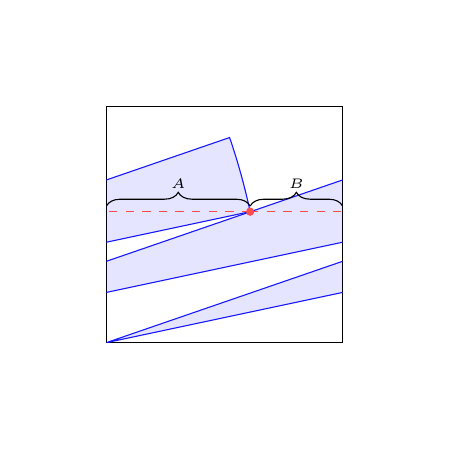
\begin{tikzpicture}
  % Constants
  \pgfmathsetmacro\b{3}
  \pgfmathsetmacro\d{8}
  \pgfmathsetmacro\t{7}
  \pgfmathsetmacro\a{12}
  \pgfmathsetmacro\x{\d*cos(\a)}
  \pgfmathsetmacro\y{\d*sin(\a)}
  % Boundary
  \path[use as bounding box] (0,0) rectangle (2+\b,2+\b);
  % Domain grids
  \draw (1,1) -- (1+\b,1) -- (1+\b,1+\b) -- (1,1+\b) -- cycle;
  % Lightcone
  \begin{scope}[shift={(1,1)}]
    \clip (0,0) rectangle(\b,\b);
    \filldraw[fill=blue,fill opacity=0.1,draw=blue!90] (0,0) -- (\a:\d) arc (\a:\a+\t:\d) -- cycle;
  \end{scope}
  \begin{scope}[shift={(1-\b,1)}]
    \clip (\b,0) rectangle(2*\b,\b);
    \filldraw[fill=blue,fill opacity=0.1,draw=blue!90] (0,0) -- (\a:\d) arc (\a:\a+\t:\d) -- cycle;
  \end{scope}
  \begin{scope}[shift={(1-2*\b,1)}]
    \clip (2*\b,0) rectangle(3*\b,\b);
    \filldraw[fill=blue,fill opacity=0.1,draw=blue!90] (0,0) -- (\a:\d) arc (\a:\a+\t:\d) -- cycle;
    % Point
    \draw[dashed,red!70] (\x,\y) -- (2*\b,\y);
    \draw[dashed,red!70] (\x,\y) -- (3*\b,\y);
    \node[circle,fill=red!70,inner sep=0,minimum size=3] at (\x,\y) {};
    \draw[decorate,decoration={brace,mirror,amplitude=5pt},yshift=2] (\x,\y) -- (2*\b,\y) node [midway,yshift=8] {\tiny $A$};
    \draw[decorate,decoration={brace,amplitude=5pt},yshift=2] (\x,\y) -- (3*\b,\y) node [midway,yshift=8] {\tiny $B$};
  \end{scope}
\end{tikzpicture}
\end{document}
}

The point in red is the intersection of the lower end of the cone's arc,
and the next highest part of the top edge of the cone. To reach that point
we must move through the two line segments $A$ and $B$. From the diagram it's clear
that $A + B = b$.

\resizebox{\textwidth}{!}{\documentclass[crop,tikz]{standalone}
\usetikzlibrary{calc}
\usetikzlibrary{arrows}
\usetikzlibrary{decorations.pathreplacing}
\begin{document}
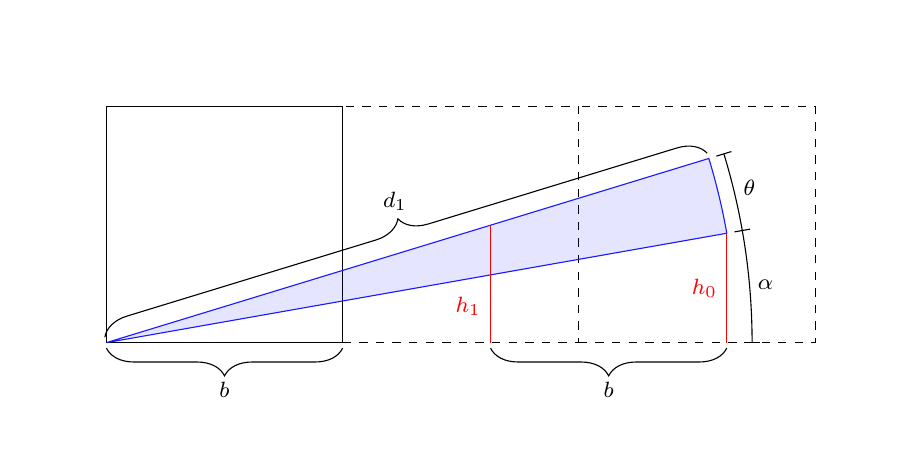
\begin{tikzpicture}
  % Constants
  \pgfmathsetmacro\b{3}
  \pgfmathsetmacro\d{8}
  \pgfmathsetmacro\t{7}
  \pgfmathsetmacro\a{10}
  \pgfmathsetmacro\x{\d*cos(\a)}
  \pgfmathsetmacro\y{\d*sin(\a)}
  \pgfmathsetmacro\w{\d*cos(\a)-\b}
  \pgfmathsetmacro\v{\w*tan(\a+\t)}
  % Boundary
  \path[use as bounding box] (0,0) rectangle (2+\b*3,2+\b);
  % Domain grids
  \draw (1,1) -- (1+\b,1) -- (1+\b,1+\b) -- (1,1+\b) -- cycle;
  \draw[dashed] (1+\b,1) -- (1+2*\b,1) -- (1+2*\b,1+\b) -- (1+\b,1+\b);
  \draw[dashed] (1+2*\b,1) -- (1+3*\b,1) -- (1+3*\b,1+\b) -- (1+2*\b,1+\b);
  % Domain size
  \draw[decorate,decoration={brace,mirror,amplitude=10pt},yshift=-2] (1,1) -- (1+\b,1) node [midway,yshift=-15] {\footnotesize $b$};
  % Lightcone
  \begin{scope}[shift={(1,1)}]
    \filldraw[fill=blue,fill opacity=0.1,draw=blue!90] (0,0) -- (\a:\d) arc (\a:\a+\t:\d) -- cycle;
    % Theta
    \draw (\a:\d+0.1) -- (\a:\d+0.3);
    \draw (\a+\t:\d+0.1) -- (\a+\t:\d+0.3);
    \draw (\a:\d+0.2) arc (\a:\a+\t:\d+0.2);
    \node at (\a+\t/2:\d+0.4) {\footnotesize $\theta$};
    % Alpha
    \draw (0:\d+0.1) -- (0:\d+0.3);
    \draw (0:\d+0.2) arc (0:\a:\d+0.2);
    \node at (\a/2:\d+0.4) {\footnotesize $\alpha$};
    % Length of d
    \draw[decorate,decoration={brace,amplitude=10pt},rotate=\a+\t,yshift=2] (0,0) -- (\d,0) node [midway,xshift=-4,yshift=16] {\footnotesize $d_1$};
    % Both h's
    \draw[decorate,decoration={brace,mirror,amplitude=10pt},yshift=-2] ({8*cos(10)-3},0) -- ({8*cos(10)},0) node [black,midway,yshift=-15] {\footnotesize $b$};
    \draw[red] (\x,0) -- (\x,\y) node [midway,left] {\footnotesize $h_0$};
    \draw[red] (\w,0) -- (\w,\v) node [midway,left,yshift=-8] {\footnotesize $h_1$};
  \end{scope}
\end{tikzpicture}
\end{document}
}

The condition that needs to be met for the optimal angle is $h_0 = h_1$.
Begin with definitions for each:

\begin{equation}
h_0 = d_1 sin(\alpha)
\end{equation}

\begin{equation}
h_1 = \left( d_1 cos(\alpha) - b \right) tan(\alpha + \theta)
\end{equation}

With those definitions, we seek a definition of $\alpha$ by equating
$h_0$ and $h_1$. This is a little complicated to find an analytical
solution, so Ridder's method is used to find a numerical solution. This
is based on $h_0 - h_1 = 0$, which gives:

\begin{equation}
b - d_1 \left( cos(\alpha) - \frac{sin(\alpha)}{tan(\alpha + \theta)} \right) = 0
\end{equation}

\section{Deep cone}

In the case where $z_{min} > 0$ we must take into consideration a cone that
looks something like this:

\resizebox{\textwidth}{!}{\documentclass[crop,tikz]{standalone}
\usetikzlibrary{calc}
\usetikzlibrary{arrows}
\usetikzlibrary{decorations.pathreplacing}
\begin{document}
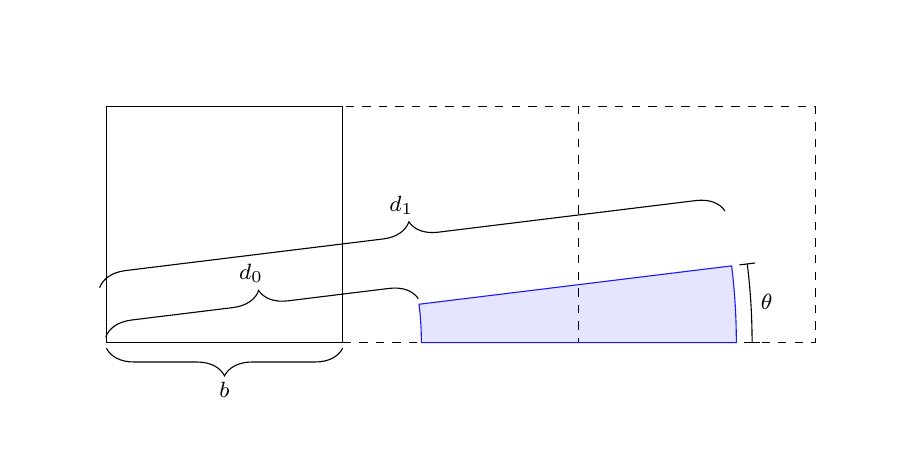
\begin{tikzpicture}
  % Constants
  \pgfmathsetmacro\b{3}
  \pgfmathsetmacro\d{8}
  \pgfmathsetmacro\c{4}
  \pgfmathsetmacro\t{7}
  \pgfmathsetmacro\a{0}
  % Boundary
  \path[use as bounding box] (0,0) rectangle (2+\b*3,2+\b);
  % Domain grids
  \draw (1,1) -- (1+\b,1) -- (1+\b,1+\b) -- (1,1+\b) -- cycle;
  \draw[dashed] (1+\b,1) -- (1+2*\b,1) -- (1+2*\b,1+\b) -- (1+\b,1+\b);
  \draw[dashed] (1+2*\b,1) -- (1+3*\b,1) -- (1+3*\b,1+\b) -- (1+2*\b,1+\b);
  % Domain size
  \draw[decorate,decoration={brace,mirror,amplitude=10pt},yshift=-2] (1,1) -- (1+\b,1) node [midway,yshift=-15] {\footnotesize $b$};
  % Lightcone
  \begin{scope}[shift={(1,1)}]
    \filldraw[fill=blue,fill opacity=0.1,draw=blue!90] (\a:\c) arc (\a:\a+\t:\c) -- (\a+\t:\d) arc (\a+\t:\a:\d) -- cycle;
    % Theta
    \draw (\a:\d+0.1) -- (\a:\d+0.3);
    \draw (\a+\t:\d+0.1) -- (\a+\t:\d+0.3);
    \draw (\a:\d+0.2) arc (\a:\a+\t:\d+0.2);
    \node at (\a+\t/2:\d+0.4) {\footnotesize $\theta$};
    % Length of c and d
    \draw[decorate,decoration={brace,amplitude=10pt},rotate=\a+\t,yshift=20] (0,0) -- (\d,0) node [midway,xshift=-4,yshift=16] {\footnotesize $d_1$};
    \draw[decorate,decoration={brace,amplitude=10pt},rotate=\a+\t,yshift=2] (0,0) -- (\c,0) node [midway,xshift=-4,yshift=16] {\footnotesize $d_0$};
  \end{scope}
\end{tikzpicture}
\end{document}
}

This actually behaves identically to the basic cone case, but requires an
offset to be applied to the origin to bring the cone back to the first
box.

\resizebox{\textwidth}{!}{\documentclass[crop,tikz]{standalone}
\usetikzlibrary{calc}
\usetikzlibrary{arrows}
\usetikzlibrary{decorations.pathreplacing}
\begin{document}
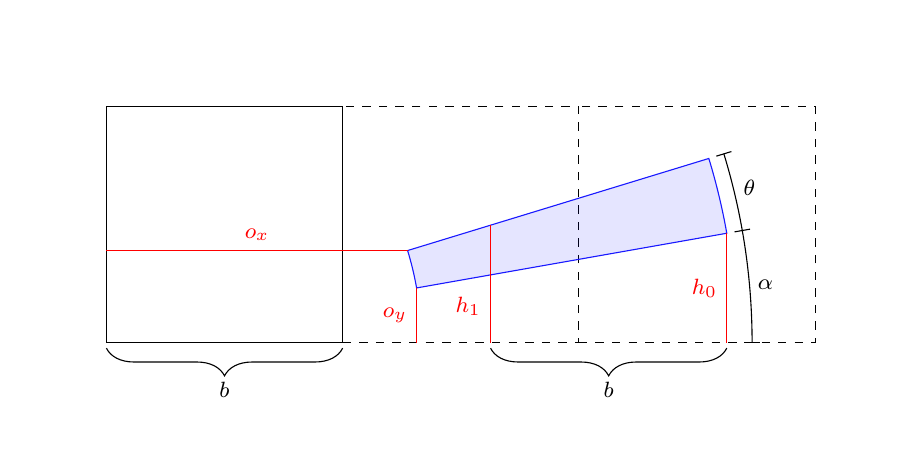
\begin{tikzpicture}
  % Constants
  \pgfmathsetmacro\b{3}
  \pgfmathsetmacro\d{8}
  \pgfmathsetmacro\c{4}
  \pgfmathsetmacro\t{7}
  \pgfmathsetmacro\a{10}
  \pgfmathsetmacro\x{\d*cos(\a)}
  \pgfmathsetmacro\y{\d*sin(\a)}
  \pgfmathsetmacro\w{\d*cos(\a)-\b}
  \pgfmathsetmacro\v{\w*tan(\a+\t)}
  \pgfmathsetmacro\ox{\c*cos(\a)}
  \pgfmathsetmacro\oy{\c*sin(\a)}
  \pgfmathsetmacro\ow{\c*cos(\a+\t)}
  \pgfmathsetmacro\ov{\c*sin(\a+\t)}
  % Boundary
  \path[use as bounding box] (0,0) rectangle (2+\b*3,2+\b);
  % Domain grids
  \draw (1,1) -- (1+\b,1) -- (1+\b,1+\b) -- (1,1+\b) -- cycle;
  \draw[dashed] (1+\b,1) -- (1+2*\b,1) -- (1+2*\b,1+\b) -- (1+\b,1+\b);
  \draw[dashed] (1+2*\b,1) -- (1+3*\b,1) -- (1+3*\b,1+\b) -- (1+2*\b,1+\b);
  % Domain size
  \draw[decorate,decoration={brace,mirror,amplitude=10pt},yshift=-2] (1,1) -- (1+\b,1) node [midway,yshift=-15] {\footnotesize $b$};
  % Lightcone
  \begin{scope}[shift={(1,1)}]
    \filldraw[fill=blue,fill opacity=0.1,draw=blue!90] (\a:\c) arc (\a:\a+\t:\c) -- (\a+\t:\d) arc (\a+\t:\a:\d) -- cycle;
    % Theta
    \draw (\a:\d+0.1) -- (\a:\d+0.3);
    \draw (\a+\t:\d+0.1) -- (\a+\t:\d+0.3);
    \draw (\a:\d+0.2) arc (\a:\a+\t:\d+0.2);
    \node at (\a+\t/2:\d+0.4) {\footnotesize $\theta$};
    % Alpha
    \draw (0:\d+0.1) -- (0:\d+0.3);
    \draw (0:\d+0.2) arc (0:\a:\d+0.2);
    \node at (\a/2:\d+0.4) {\footnotesize $\alpha$};
    % Length of c and d
    % \draw[decorate,decoration={brace,amplitude=10pt},rotate=\a+\t,yshift=20] (0,0) -- (\d,0) node [midway,xshift=-4,yshift=16] {\footnotesize $d_1$};
    % \draw[decorate,decoration={brace,amplitude=10pt},rotate=\a+\t,yshift=2] (0,0) -- (\c,0) node [midway,xshift=-4,yshift=16] {\footnotesize $d_0$};
    % Both h's
    \draw[decorate,decoration={brace,mirror,amplitude=10pt},yshift=-2] ({8*cos(10)-3},0) -- ({8*cos(10)},0) node [black,midway,yshift=-15] {\footnotesize $b$};
    \draw[red] (\x,0) -- (\x,\y) node [midway,left] {\footnotesize $h_0$};
    \draw[red] (\w,0) -- (\w,\v) node [midway,left,yshift=-8] {\footnotesize $h_1$};
    % Offsets
    \draw[red] (\ox,0) -- (\ox,\oy) node [midway,left] {\footnotesize $o_y$};
    \draw[red] (\ow,\ov) -- (0,\ov) node [midway,above] {\footnotesize $o_x$};
  \end{scope}
\end{tikzpicture}
\end{document}
}

The values for $o_x$ and $o_y$ are easily calculated:

\begin{equation}
o_x = d_0 cos(\theta + \alpha)
\end{equation}

\begin{equation}
o_y = d_0 sin(\alpha)
\end{equation}

\section{Example: Real values}

The first example is a real world basic cone with parameters:

\begin{equation}
\begin{split}
b &= 500 \\
\theta &= 8\degree \\
d_0 &= 0 \\
d_1 &= 0.45
\end{split}
\end{equation}

\resizebox{\textwidth}{!}{\documentclass[crop,tikz]{standalone}
\usetikzlibrary{calc}
\usetikzlibrary{arrows}
\usetikzlibrary{decorations.pathreplacing}
\begin{document}
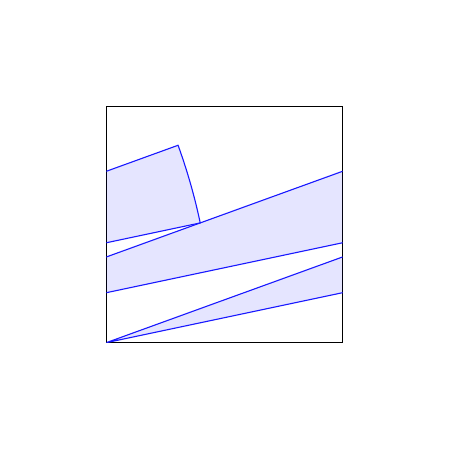
\begin{tikzpicture}
  % Constants
  \pgfmathsetmacro\b{3}
  \pgfmathsetmacro\d{7.3506}
  \pgfmathsetmacro\t{8}
  \pgfmathsetmacro\a{11.938}
  % Boundary
  \path[use as bounding box] (0,0) rectangle (2+\b,2+\b);
  % Domain grids
  \draw (1,1) -- (1+\b,1) -- (1+\b,1+\b) -- (1,1+\b) -- cycle;
  % Lightcone
  \begin{scope}[shift={(1,1)}]
    \clip (0,0) rectangle(\b,\b);
    \filldraw[fill=blue,fill opacity=0.1,draw=blue!90] (0,0) -- (\a:\d) arc (\a:\a+\t:\d) -- cycle;
  \end{scope}
  \begin{scope}[shift={(1-\b,1)}]
    \clip (\b,0) rectangle(2*\b,\b);
    \filldraw[fill=blue,fill opacity=0.1,draw=blue!90] (0,0) -- (\a:\d) arc (\a:\a+\t:\d) -- cycle;
  \end{scope}
  \begin{scope}[shift={(1-2*\b,1)}]
    \clip (2*\b,0) rectangle(3*\b,\b);
    \filldraw[fill=blue,fill opacity=0.1,draw=blue!90] (0,0) -- (\a:\d) arc (\a:\a+\t:\d) -- cycle;
  \end{scope}
\end{tikzpicture}
\end{document}
}

The second example is the same as the first, but with a minimum
distance for the cone:

\begin{equation}
\begin{split}
b &= 500 \\
\theta &= 8\degree \\
d_0 &= 0.2 \\
d_1 &= 0.45
\end{split}
\end{equation}

\resizebox{\textwidth}{!}{\documentclass[crop,tikz]{standalone}
\usetikzlibrary{calc}
\usetikzlibrary{arrows}
\usetikzlibrary{decorations.pathreplacing}
\begin{document}
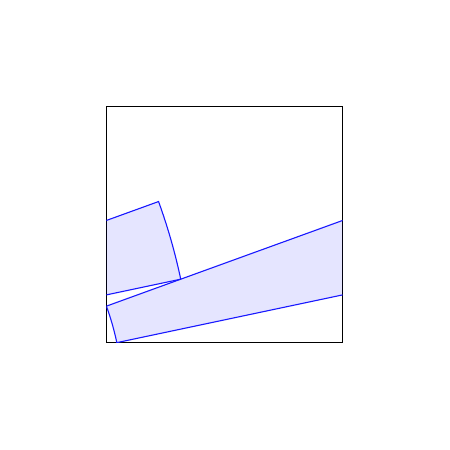
\begin{tikzpicture}
  % Constants
  \pgfmathsetmacro\b{3}
  \pgfmathsetmacro\d{7.3506}
  \pgfmathsetmacro\c{3.4548}
  \pgfmathsetmacro\t{8}
  \pgfmathsetmacro\a{11.938}
  \pgfmathsetmacro\ox{\c*cos(\a+\t)}
  \pgfmathsetmacro\oy{\c*sin(\a)}
  % Boundary
  \path[use as bounding box] (0,0) rectangle (2+\b,2+\b);
  % Domain grids
  \draw (1,1) -- (1+\b,1) -- (1+\b,1+\b) -- (1,1+\b) -- cycle;
  % Lightcone
  \begin{scope}[shift={(1-\ox,1-\oy)}]
    \clip (\ox,\oy) rectangle(\b+\ox,\b+\oy);
    \filldraw[fill=blue,fill opacity=0.1,draw=blue!90] (\a:\c) arc (\a:\a+\t:\c) -- (\a+\t:\d) arc (\a+\t:\a:\d) -- cycle;
  \end{scope}
  \begin{scope}[shift={(1-\b-\ox,1-\oy)}]
    \clip (\b+\ox,\oy) rectangle(2*\b+\ox,\b+\oy);
    \filldraw[fill=blue,fill opacity=0.1,draw=blue!90] (\a:\c) arc (\a:\a+\t:\c) -- (\a+\t:\d) arc (\a+\t:\a:\d) -- cycle;
  \end{scope}
  %% \begin{scope}[shift={(1-2*\b,1)}]
  %%   \clip (2*\b,0) rectangle(3*\b,\b);
  %%   \filldraw[fill=blue,fill opacity=0.1,draw=blue!90] (\a:\c) arc (\a:\a+\t:\c) -- (\a+\t:\d) arc (\a+\t:\a:\d) -- cycle;
  %%   %% \filldraw[fill=blue,fill opacity=0.1,draw=blue!90] (0,0) -- (\a:\d) arc (\a:\a+\t:\d) -- cycle;
  %% \end{scope}
\end{tikzpicture}
\end{document}
}

\end{document}
